\documentclass{article}
%\url{https://tex.stackexchange.com/q/440528/86}
\usepackage{tikz}
\usetikzlibrary{knots}

\begin{document}

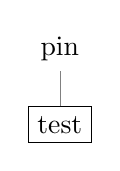
\begin{tikzpicture}
\node[draw,pin={[node contents={pin}]}] (a) {test};
\end{tikzpicture}

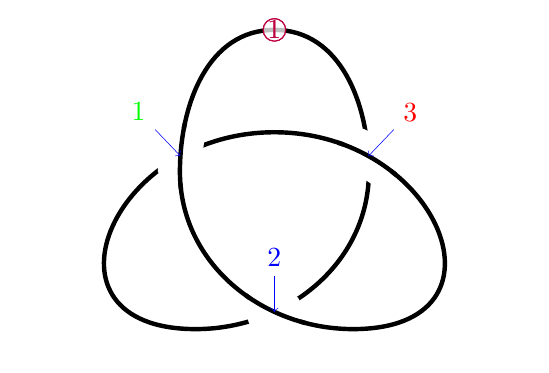
\begin{tikzpicture}
\begin{knot}[
  draft mode=crossings,
  clip width=10pt,
  consider self intersections,
  end tolerance=1pt,
  draft/crossing 3 label/.style={
    text=red,
    pin position=45,
  },
  draft/crossing 1 label/.style={
    text=green,
    pin position=135,
  }
]
\strand[ultra thick]
(0,0.3) to[out=180,in=90]
(-1.2,-1.5) to[out=-90,in=180]
(1,-3.5) to[out=0,in=0,looseness=2]
(0,-1) to[out=180,in=180,looseness=2]
(-1,-3.5) to[out=0,in=-90]
(1.2,-1.5) to[out=90,in=0] (0,0.3);
\end{knot}
\end{tikzpicture}

\end{document}
